\documentclass[french, 12pt]{article}%

\usepackage[utf8]{inputenc}  
\usepackage[francais]{babel}
\usepackage{appendix}
\usepackage{pdfpages} 
\usepackage{eurosym}
%\usepackage[T1]{fontenc}

%%%%%%%%%%%%%%%%%%%%%%%%%%%%%%%%%%%%%%%%%%%%%%%%%%%%%%%%%
\newcommand{\itemE}{\item[$\bullet$]}
\newcommand{\titreSeq}{Docker}
\newcommand{\lycee}{Lycée de Brocéliande}
\newcommand{\classSeq}{SNIR1 }
\newcommand{\matiereSeq}{IR}      
\newcommand{\numSeq}{Cyber}
\newcommand{\numAct}{01}
\newcommand{\objSeance}{Apprendre à utiliser des containers}

\newcommand{\moySeq}{\begin{itemize}	
\itemE Machine avec OS Linux ou Windows
\end{itemize}}

\newcommand{\compSeq}{\begin{itemize}
\item  
\end{itemize}}
%%%%%%%%%%%%%%%%%%%%%%%%%%%%%%%%%%%%%%%%%%%%%%%%%%%%%%%%%%

%%%%%%%%%%%%%%%%%%%%%%%%%%%%%%%%%%%%%%%%%%%%%%%%%%%%%%%%
%%%%Algo
\usepackage[linesnumbered, french]{algorithm2e}
\SetKwFor{For}{Pour}{faire}{fin}
\SetKwFor{While}{Tant que}{faire}{fin}%
\SetKw{KwTo}{à}
\SetKw{KwPas}{par pas de}
\SetKw{KwRet}{Retourne}
\SetKwProg{Fn}{Fonction }{ arguments }{fin}
\SetKwRepeat{Repeat}{Répéter}{jusqu'à}%
\SetKwIF{If}{ElseIf}{Else}{Si}{alors}{Sinon si}{Sinon}{Fin}


\usepackage{listings} %%%%Présenration code source
\lstset{language=C++,
    %numbers=left,
    %stepnumber=1,
    %showstringspaces=false,
    %tabsize=1,
    %breaklines=true,
    %breakatwhitespace=false,
    basicstyle=\footnotesize,
    keywordstyle=\color{blue}\footnotesize,
    stringstyle=\color{red}\footnotesize,
    commentstyle=\color{green}\footnotesize,
    morecomment=[l][\color{magenta}]{\#}
    }
\lstdefinestyle{commande}{
  basicstyle=\ttfamily\footnotesize,
  keywordstyle=\color{blue},
  commentstyle=\color{gray},
  %numbers=left,
  %numberstyle=\tiny\color{gray},
  numbersep=5pt,
  breaklines=true,
  frame=single,
  backgroundcolor=\color{lightgray!10},
  %captionpos=b,
  %caption=\lstname   
    extendedchars=true,
    literate={é}{{\'e}}1
             {è}{{\`e}}1
             {à}{{\`a}}1
             {ç}{{\c{c}}}1
             {✔}{{\checkmark}}1,
}
%\usepackage[T1]{fontenc}


% Margins
\topmargin=-0.45in
\evensidemargin=0in
\oddsidemargin=0in
\textwidth=6.5in
\textheight=9.0in
\headsep=0.25in 


\linespread{1.1} 
\usepackage{amsmath}%
\usepackage{amsfonts}%
\usepackage{amssymb}%
\usepackage{graphicx}
\usepackage{lastpage}
\usepackage{enumitem}

%\usepackage[T1]{fontenc}    
\usepackage{multirow}
\usepackage{lscape}
\usepackage[colorlinks = true,
            linkcolor = blue,
            urlcolor  = blue,
            citecolor = blue,
            anchorcolor = blue]{hyperref}
\usepackage{array}
\usepackage{mwe}
%-------------------------------------------
\newtheorem{theorem}{Theorem}
\newtheorem{summary}[theorem]{Summary}
\newenvironment{proof}[1][Proof]{\textbf{#1.} }{\ \rule{0.5em}{0.5em}}
\newcommand{\paraL}[1]{\tiny\noindent\rule{1.0\linewidth}{0.5pt}\paragraph*{#1}\  \normalsize}


\usepackage{xcolor}

\usepackage{colortbl}
\definecolor{vert_capet}{RGB}{191,255,191}	
\definecolor{bleu_snir}{RGB}{101,191,179}	
\setlength{\doublerulesep}{\arrayrulewidth}
%-------------------------------------------
%%%%%%%%%%%%%%%%%%%%%%%%%%%%%%%%%%%%%%%%%%%%%
\usepackage[framemethod=tikz]{mdframed}
\usepackage{tikz, xcolor, lipsum}
\makeatletter
\mdfsetup{skipabove=\topskip,skipbelow=\topskip}

\tikzset{titre_bleu_snir/.style =
	{draw=bleu_snir, line width=1.5pt, fill=white,
	rectangle, rounded corners, right,minimum height=2em}}
\newcommand{\titreencadre}{Titre}
\makeatletter
\mdfdefinestyle{encadrestyle}{%
	linewidth=1.5pt,roundcorner=5pt,linecolor=bleu_snir,
	apptotikzsetting={\tikzset{mdfbackground/.append style ={%
		fill=white}}},
	frametitlefont=\bfseries,
	singleextra={%
		\node[titre_bleu_snir,xshift=2em] at (P-|O) %
			{~\mdf@frametitlefont{\titreencadre}\hbox{~}};},
	firstextra={%
		\node[titre_bleu_snir,xshift=2em] at (P-|O) %
		{~\mdf@frametitlefont{\titreencadre}\hbox{~}};},
	}
\mdfdefinestyle{encadresanstitrestyle}{%
	linewidth=1.5pt,roundcorner=5pt,linecolor=bleu_snir
	apptotikzsetting={\tikzset{mdfbackground/.append style ={%
		fill=yellow!20}}},
	}

\newenvironment{encadre}[1]{\renewcommand{\titreencadre}{#1}
	\begin{mdframed}[style=encadrestyle]
	\vspace{0.5\baselineskip}
	}{%
	\end{mdframed}}

\newenvironment{encadresanstitre}{
	\begin{mdframed}[style=encadresanstitrestyle]
	}{%
	\end{mdframed}}
\makeatother
\usepackage{colortbl}
\definecolor{vert_capet}{RGB}{191,255,191}	
\definecolor{bleu_snir}{RGB}{101,191,179}	
\setlength{\doublerulesep}{\arrayrulewidth}
%-------------------------------------------
\usepackage{comment}
%%%%%%%%%%%%%%%%%%%%%%%%%%%%%%%
\newif\ifPROF

%\def\PourProf{0}
\ifdefined\PourProf
  \PROFtrue
  \newenvironment{corr}{\begingroup \color{red}}{\normalcolor \endgroup}
\else
  \PROFfalse
  \newenvironment{corr}{\begingroup \color{white}}{\normalcolor \endgroup}
\fi
%\PROFtrue

%%%%%%%%%%%%%%%%%%%%%%%%%%%%%%%%%%%%




%%%Note et pied de page
\usepackage{fancybox}
\usepackage{fancyhdr}
\usepackage[a4paper,margin=2.5cm,bottom=2cm,headheight=2cm]{geometry}
\pagestyle{fancy}
\fancyhead[R]{
\includegraphics[scale=0.3]{logo_CIEL.png}}
\fancyhead[C]{Prénom}
\fancyhead[L]{Nom}
\fancyfoot[C]{Page \thepage/\pageref{LastPage}}
\fancyfoot[L]{\classSeq ~\matiereSeq}
\fancyfoot[R]{Formation \numSeq  ~ r \numAct}
\renewcommand{\headrulewidth}{1pt}
%%%Note et pied de page 



\begin{document}
\lstset{basicstyle = \ttfamily,columns=fullflexible}
\title{\titreSeq\\
 
\includegraphics[scale=0.5]{logo_CIEL.png}\\
}
\author{\lycee}
\date{}%\today}
%\maketitle

\noindent\begin{tabular}{!{\vrule width 1.5pt}m{0.7\linewidth}!{\vrule width 1.5pt}m{0.2\linewidth}!{\vrule width 1.5pt}}
\hline\hline
\cellcolor{vert_capet}
\begin{center}
	\Large\textbf{\titreSeq}  
\end{center}
  & 

\begin{minipage}{1.0\linewidth}
  \vspace*{0.1cm} 
\centering
\includegraphics[scale=0.2]{logo_lycee.jpg}

{\tiny\today}
  \vspace*{0.1cm} 
\end{minipage}\\ \hline\hline

\multicolumn{2}{!{\vrule width 1.5pt}l!{\vrule width 1.5pt}}{
\begin{minipage}{14cm}
\vspace*{0.1cm} 
\textbf{Objectif} : \objSeance
\vspace*{0.1cm} 
\end{minipage}} \\ \hline\hline

\multicolumn{2}{!{\vrule width 1.5pt}l!{\vrule width 1.5pt}}{
\begin{minipage}{14cm}
\vspace*{0.1cm} 
\textbf{Moyens} : 
\moySeq
\vspace*{0.1cm} 
\end{minipage}} \\ \hline\hline
%
%\multicolumn{2}{!{\vrule width 1.5pt}l!{\vrule width 1.5pt}}{
%\begin{minipage}{14cm}
%\vspace*{0.1cm}
%\tiny
%Compétences attendues :
%\compSeq
%\vspace*{0.1cm}
%\end{minipage}}
%\normalsize \\ \hline\hline
\end{tabular}

%%%%%%%%%%%%%%%%%%%%%%%%%%%%%%%%%%%%%%%%%%%%%%%%%%%%%%%%%%%%%%%%%%%%%%%%%%%%%%%%
\vspace{0.25cm}

%%%%%%%%%%%%%%%%%%%%%%%%%%%%%%%%%%%%%%%%%%%%%%%%%%%%%%%%%%%%%%%%%%%%%%%%%%%%%%%%%%%%%%%%%%%%%%%
%%%%%%%%%%%%%%%%%%%%%%%%%%%%%%  DEBUT %%%%%%%%%%%%%%%%%%%%%%%%%%%%%%%%%%%%%%%%%%%%%%%%%%%%%%%%%
%%%%%%%%%%%%%%%%%%%%%%%%%%%%%%%%%%%%%%%%%%%%%%%%%%%%%%%%%%%%%%%%%%%%%%%%%%%%%%%%%%%%%%%%%%%%%%%

\section{Objectif }

Ce document a pour objectif de démystifier le principe des container docker avec la mise en place d'un serveur \textbf{Nginx} avec \textbf{Docker}. 

\begin{encadre}{Commandes utiles}
\textbf{Vous trouverez en annexe \ref{lbl_CommandeUtiles} un ensemble de commandes utiles pour exploiter pleinement le containers.}
\end{encadre}
\begin{center}
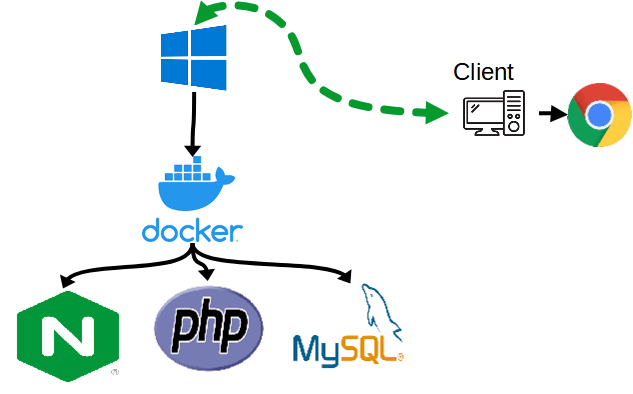
\includegraphics[scale=0.6]{./ressource/schema_docker}
\end{center}



\section{Présentation de docker}

Les conteneurs sont semblables à une forme de virtualisation qui permet d'isoler les applications. Il reste cependant différent de la virtualisation.
Toutes les fonctionnalités de la virtualisation du système d'exploitation ne sont pas disponibles. Il y a seulement les ressources nécessaires. Il en résulte un temps de démarrage plus rapide ! 
Un développeur peut spécifier les ressources dont il a besoin, le système d'exploitation dont il a besoin pour exécuter l'application et il n'a pas à se soucier des dépendances puisque le conteneur s'en occupe.

\paragraph{Machines virtuelles vs conteneurs} Une machine virtuelle (VM) est comme une copie d'un ordinateur physique réel utilisant une technologie d’hyperviser proche de l’émulation. 

Plusieurs VM peuvent fonctionner sur le même matériel physique. En revanche, les conteneurs se trouvent installés sur un serveur physique et son système d'exploitation hôte, voir dans une VM.
Chaque conteneur partage le noyau de l'OS hôte cependant les binaires et les bibliothèques nécessaires à l'exécution de ces applications lui sont spécifiques.
  
On peut partager l’image d’un conteneur (une copie à un instant t, re-executable).  On peut donc diffuser des logiciels, ou des données via un conteneur dans une version fixe.  Ainsi à partir des mêmes sources répliquées, les autres utilisateurs obtiendront les mêmes résultats. 


\begin{center}
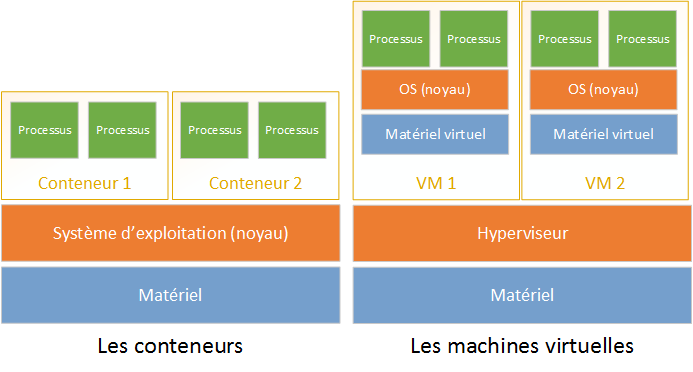
\includegraphics[scale=0.6]{./ressource/conteneur_vs_mv.png}
\end{center}

\paragraph{Architecture générale} Docker utilise une architecture client-serveur, qui implique les trois principaux composants.   
\begin{itemize}
\itemE le client Docker, 
\itemE le deamon Docker 
\itemE le registre Docker (dockerhub par défaut).
\end{itemize}
  
\begin{encadre}{Daemon}
Type de programme informatique, un processus ou un ensemble de processus qui s'exécute en arrière-plan plutôt que sous le contrôle direct d'un utilisateur.
\end{encadre}  
  
Le client Docker communique avec le démon Docker, qui se charge de construire, d'exécuter et de distribuer les conteneurs Docker. 


\begin{encadre}{Container}
Ensemble de processus logiciels léger et indépendant, regroupant tous les fichiers nécessaires à l’exécution des processus : code, runtime, outils système, bibliothèque et paramètres.
\end{encadre}

Le client et le démon Docker peuvent fonctionner sur le même système ou connecter un client à un démon Docker distant. 

 Les conteneurs peuvent avoir différents états : 
 
 \begin{center}
 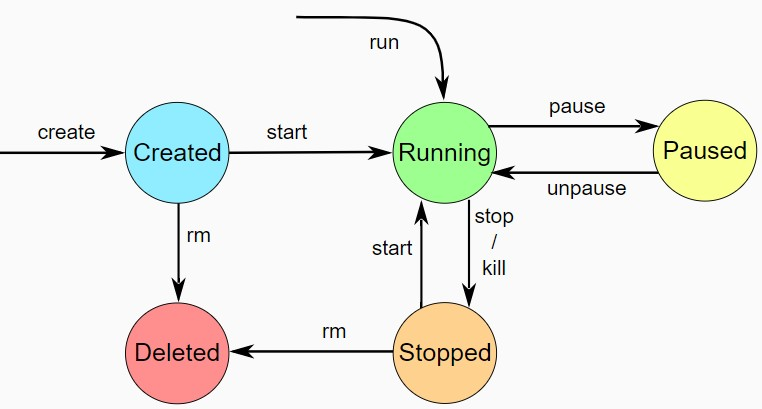
\includegraphics[scale=0.7]{./ressource/docker_etat}
 \end{center}

Les données stockées à l'extérieur du conteneur peuvent être utilisées même si le conteneur n'existe plus. Cependant, pour cela il est nécessaire de monter les données à l'extérieur du conteneur.


\section{Installation de docker }

Pour l'installation, il est nécessaire de suivre le tutoriel accessible via ce lien : \href{https://practicalprogramming.fr/install-docker-windows/}{Tuto docker}.

\paragraph{Remarque : } Cette étape n'a pas de difficulté. 

\paragraph{Docker Hub } : est un service fourni par Docker. vous pouvez le comparer à GitHub, mais spécialisé dans le stockage d'image pour Docker.

Pour utiliser Docker (et donc pour la suite), il est recommandé de créer un compte sur le \href{https://hub.docker.com/}{Docker Hub}. 

\section{Premier pas}

\subsection{Commandes}
Cette partie a pour objectif de vous familiariser avec l'interface en \textbf{ligne de commande} qui permet de discuter avec le daemon Docker 


Depuis un terminal, si vous exécutez la commande docker, vous obtiendrez une liste de commandes exécutables, que voici :


\begin{lstlisting}
$ docker
...
Commands:
    attach    Attach to a running container
    build     Build an image from a Dockerfile
    commit    Create a new image from a container s changes
	....
    login     Register or log in to a Docker registry server
    logout    Log out from a Docker registry server
    logs      Fetch the logs of a container
    port      Lookup the public-facing port that is NAT-ed to PRIVATE_PORT
    pause     Pause all processes within a container
    ps        List containers
    pull      Pull an image or a repository from a Docker registry server
    push      Push an image or a repository to a Docker registry server
    restart   Restart a running container
    rm        Remove one or more containers
    rmi       Remove one or more images
    run       Run a command in a new container
    ....
\end{lstlisting}

Grâce à ces différentes commandes, vous pouvez facilement gérer vos containers et vos images.  Nous verrons au cours de cette activité, les commandes les plus pratiques.


\subsection{Images}

\begin{encadre}{Image}
Une image est un container statique. On pourrait comparer une image à une capture d'un container à un moment donné. Lorsqu'on souhaite travailler avec un container, on déclare forcément un container à partir d'une image.
\end{encadre}

Vous pouvez à tout moment voir votre « bibliothèque » d'images avec la commande "docker images". Vous verrez, au fil des projets, vous aurez de plus en plus d'images. Utilisables comme "moules" à votre guise pour débuter vos projets ou, à minima, vos nouveaux containers.

Pour voir votre bibliothèque d'images :

\shadowbox{\begin{lstlisting}[language=sh]
> docker images
REPOSITORY              TAG       IMAGE ID       CREATED        SIZE
test_php                latest    214adac37e21   24 hours ago   449MB
nginx                   latest    2b7d6430f78d   3 days ago     142MB
mysql/mysql-server      latest    eb5713a2c247   4 weeks ago    428MB
phpmyadmin/phpmyadmin   latest    4a4023c7e22a   3 months ago   510MB
\end{lstlisting}}

Sur ma machine, il y a 4 images (que vous utiliserez pas la suite).

\vspace{0.5cm}


Il existe une plateforme maintenue par Docker sur laquelle tout le monde peut \verb?pusher? et \verb?puller? des images. C'est un peu comme le GitHub des images Docker (vous verrez cela durant votre formation). Il existe des images officielles pour tout et n'importe quoi ! Cette bibliothèque géante partagée, c'est le Docker Hub Registry !

\begin{encadre}{Push}
Commande 'générique' permettant de \textbf{déposer} des fichiers sur un dépôt. 
\end{encadre}
\begin{encadre}{Pull}
Commande 'générique' permettant de \textbf{récupérer} des fichiers sur un dépôt. 
\end{encadre}

\begin{center}
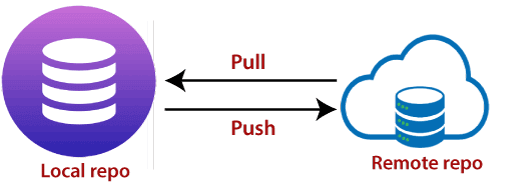
\includegraphics[scale=0.7]{./ressource/pull_push.png}
\end{center}





\subsection{Hello World}

Pour valider le fonctionnement de Docker (et comme toujours en informatique), vous allez récupérer une image de Hello world et la lancer sur votre machine. Pour cela : 

\begin{itemize}
\itemE Allez sur \verb?hub docker?
\itemE Cherchez l'image de \verb?Hello world?
\itemE Télécharger l'image
\end{itemize}

\shadowbox{\begin{lstlisting}[language=sh]
docker pull hello-world
\end{lstlisting}}

\begin{itemize}
\itemE Vérifier avec la commande adapté que votre image a bien été téléchargée.
\end{itemize}


\paragraph{Commande run}. Cette commande permet de créer un nouveau container et télécharger son image si elle n’est pas déjà en local. Pour créer et exécuter un container, il faut utiliser cette commande de la manière suivante 

\shadowbox{\begin{lstlisting}[language=sh]
docker run hello-world
\end{lstlisting}}

Un grand nombre d'option que l'on verra par la suite permet de configurer le lancement des dockers (liste non-exhaustive) :
\begin{itemize}
\itemE \verb?-d? : lance le container en arrière plan.
\itemE \verb?-t? : alloue terminal
\itemE \verb?-p 8080:80? : redirige un port interne du container vers un port
local
\itemE \verb?-rm? : supprime le container à la sortie
\itemE \verb?-v rep_local/rep_container? : lie un répertoire local à un répertoire du container
\itemE ...
\end{itemize}



\textbf{Appeler votre très cher professeur si vous avez des difficultés.}

\vspace{0.5cm}

Le résultat d'exécution doit être le suivant :  

\begin{lstlisting}
Hello from Docker!
This message shows that your installation appears to be working correctly.
...
...
\end{lstlisting}

Si c'est le cas : Bravo, vous pouvez passer à la suite.


\section{Dockerfile}




\begin{minipage}{0.6\linewidth}
Vous maitrisez maintenant les containers Docker. Il va falloir passer à l'étape suivante : installer un container 'utile'. Vous voudriez avoir à disposition un environnement linux avec la chaine de compilation \textbf{gcc} (vue en début d'année). Pour cela, il y a plusieurs solutions.  

\end{minipage}
\begin{minipage}{0.39\linewidth}
\begin{center}

\includegraphics[scale=0.05]{./ressource/gcc}
\end{center}
\end{minipage}
\begin{itemize}
\itemE Vous installer cygwin sur windows pour émuler un système Linux $\Rightarrow$ Lourd et peu stable
\itemE Vous installer une machine virtuelle linux et y installer gcc  $\Rightarrow$ Lourd et mais stable
\itemE Vous utiliser toutes les fonctionnalités des containers docker $\Rightarrow$ \textbf{léger et stable}
\end{itemize}

\subsection{1er test}


Voici la procédure que vous devez réaliser sur la machine hôte (dans un powershell sous Windows) : 
\begin{enumerate}
\item Installer l'image de Ubuntu (vous pouvez aller voir sa description sur docker hub). Pour cela dans un powershell Windows taper la commande suivante : 
\end{enumerate}

\shadowbox{\begin{lstlisting}[language=sh]
docker pull ubuntu
\end{lstlisting}}

\begin{enumerate}[resume]
\item Créer et lancer l'image d'ubuntu. Profiter en pour nommer le container (dans l'exemple le container est nommé ubuntuPV)
\end{enumerate}

\shadowbox{\begin{lstlisting}[language=sh]
docker run -d -t --name ubuntuPV ubuntu
\end{lstlisting}}
 
 \begin{enumerate}[resume]
\item Vérifier que votre container est bien lancé : 
\end{enumerate}

\shadowbox{\begin{lstlisting}[language=sh]
docker ps 
\end{lstlisting}}

Vous devez voir votre container.

\begin{enumerate}[resume]
\item Lancer un terminal bash de votre container ubuntu : 
\end{enumerate}


\shadowbox{\begin{lstlisting}[language=sh]
docker exec -it ubuntuPV bash
\end{lstlisting}}
 
 
\begin{enumerate}[resume]
\item Dans le terminal Ubuntu, vérifier l'accès à gcc : 
\end{enumerate}


\shadowbox{\begin{lstlisting}[language=sh]
gcc -v
\end{lstlisting}} 
 
\begin{enumerate}[resume]
\item Y-a-t'il un problème? 
\end{enumerate}

\subsection{Création de votre propre image}

Comme vous avez pu le constater, l'image officiel d'Ubuntu n'inclut pas gcc. Vous allez maintenant apprendre à créer une image avec les éléments que vous souhaitez : 
\begin{itemize}
\itemE GCC
\itemE vim (comme cela vous aurez accès à un éditeur de texte sur cette distribution). 
\end{itemize}

Pour cela, vous allez utiliser un dockefile. 

\begin{encadre}{Dockerfile}
Un Dockerfile est un simple fichier texte placé sur la machine hôte regroupant l'ensemble des commandes pour construire l'image. Une fois l'image personnelle créée, vous pourrez créer une instance exécutable de cette image.
\end{encadre}

\begin{center}
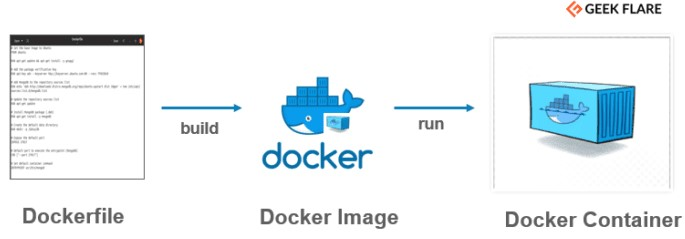
\includegraphics[scale=0.7]{./ressource/docker_file_schema.jpg}
\end{center}

\begin{enumerate}
\item Ainsi, la première étape est de créer dans un répertoire de votre choix sur la machine hôte un fichier nommé "Dockerfile" (sans extension). Il contiendra toutes les instructions pour créer votre image. 
\end{enumerate}

Le fichier Dockerfile doit contenir les instructions qui suivent : 
\begin{enumerate} [resume]
\item La première instruction obligatoire doit indiquer l'image de base
\end{enumerate}

\shadowbox{\begin{lstlisting}[language=sh]
FROM ubuntu:latest
\end{lstlisting}}

\begin{enumerate}[resume]
\item Ensuite, il faut écrire l'instruction \verb?RUN? pour exécuter une commande dans notre container. Vous voulez : 	
	\begin{itemize}
	\itemE Mettre à jour, 
	\itemE Installer GCC
	\itemE Installer vim
	\end{itemize}
\end{enumerate}

\shadowbox{\begin{lstlisting}[language=sh]
RUN apt-get update -yq \
&& apt-get install gcc -yq \
&& apt-get install vim -yq \
&& apt-get clean -y
\end{lstlisting}}

\begin{enumerate}[resume]
\item Vous voulez aussi que votre répertoire de travail par défaut (au lancement de l'image) soit  : \verb?/usr/src/?
\end{enumerate}

\shadowbox{\begin{lstlisting}[language=sh]
WORKDIR /usr/src
\end{lstlisting}}

Il existe beaucoup d'autres options pour configurer votre image (que nous verrons pas dans cette activité). 

\begin{enumerate}[resume]
\item Vous allez maintenant créer votre image. Placer dans le répertoire du fichier et exécuter la commande 
\end{enumerate}


\shadowbox{\begin{lstlisting}[language=sh]
  docker build -t imageperso .
\end{lstlisting}}

Cette commande construit l'image de ubuntu+Gcc+Vim et la nomme \verb?imageperso?.


Vous avez maintenant construit une nouvelle image que vous pouvez utiliser, partager,....

\begin{enumerate}[resume]
\item Vérifier avec les commandes appropriés que vous pouvez créer un container permettant d'avoir un environnement Linux avec gcc et vim
\end{enumerate}


\subsection{Fichiers partagés}


Vous avec un container fait 'maison' avec un environnement de développement gcc. Une question reste en suspend : commet faire pour que mon container est accès aux fichiers de mon ordinateur? Rien de plus simple, il suffit de créer un parage de fichier entre l'hote et docker. 

\begin{enumerate}
\item Dans le répertoire du dockerfile, créer un sous-répertoire nommé src (pour source) contenant un fichier C helloworld.c. Ce fichier contient le code source pour afficher helloworld.
\end{enumerate}

\begin{enumerate}[resume]
\item Créer et lancer le container (instance de l'image \verb?imageperso?) grâce à la commande ci-dessous. 
\end{enumerate}

\shadowbox{\begin{lstlisting}[language=sh]
docker run -d -t -v C:\Users\Pierre\...\src:/usr/src/
	 --name containerPV imageperso
\end{lstlisting}}



Le partage de fichier se fait grâce à l'option \verb?-v [repertoire hote]: [repertoire docker]?. Le nom du container est \verb?containerPV? (vous pouvez bien sur le changer). L'image d'origine du container est \verb?imageperso?.


Vous pouvez maintenant tester le bon fonctionnement de gcc (compilateur C)
\begin{enumerate}[resume]
\item Ouvrer un shell de votre container  (invité de commande)
\end{enumerate}

\shadowbox{\begin{lstlisting}[language=sh]
docker exec -it containerPV bash
\end{lstlisting}}

\begin{enumerate}[resume]
\item Vérifier que votre fichier partagé est présent  (\verb?hello_wrold.c?)
\end{enumerate}

\shadowbox{\begin{lstlisting}[language=sh]
ls
\end{lstlisting}}

\begin{enumerate}[resume]
\item Compiler le code source C avec la commande
\end{enumerate}

\shadowbox{\begin{lstlisting}[language=sh]
gcc hello_world.c -o progExecutable
\end{lstlisting}}

\begin{enumerate}[resume]
\item Vous venez alors de créer un programme nommé \verb?progExecutable?. Pour l'exécuter il suffit de taper
\end{enumerate}

\shadowbox{\begin{lstlisting}[language=sh]
./progExecutable
\end{lstlisting}}

Normalement, un message 'hello world' apparaît. C'est que tout fonctionne.

\begin{enumerate}[resume]
\item Vous pouvez quitter le container en tapant 
\end{enumerate}

\shadowbox{\begin{lstlisting}[language=sh]
exit
\end{lstlisting}}

Il reste toujours en exécution même si vous n'avez plus de visuel sur le terminale. 

\begin{enumerate}[resume]
\item Pour retourner dans le container, il est possible de refaire la commande suivante.
\end{enumerate}

\shadowbox{\begin{lstlisting}[language=sh]
docker exec -it containerPV bash
\end{lstlisting}}



\section{Orchestration des containers}

Vous souhaiteriez avoir un serveur LEMP constitué de : 
\begin{itemize}
\itemE \textbf{Nginx}
\itemE \textbf{PHP}
\itemE \textbf{mysql}
\itemE \textbf{Phpmyadmin}
\end{itemize}

Vous pouvez créer et lancer des containers 'à la main' comme vu précédemment. Vous verrez si vous essayer que ce n'est pas le plus pratique. Il existe une solution appropriée : Docker compose. 


\begin{encadre}{Docker compose}
Docker Compose va vous permettre d'orchestrer vos conteneurs, et ainsi de simplifier vos déploiements sur de multiples environnements. Docker Compose est un outil écrit en Python qui permet de décrire, dans un fichier YAML, plusieurs conteneurs comme un ensemble de services.
\end{encadre} 

En résumé, il suffit de configurer correctement un fichier nommé : \verb?docker-compose.yml? pour pouvoir lancer un ensemble de container.

\subsection{1er pas : Nginx}

Le 1re test est de regarder uniquement si vous arrivez à orchestrer  avec docker compose un unique container composer uniquement de \textbf{Nginx}. 

\begin{enumerate}
\item Préparer vous un répertoire de travail contenant un fichier nommé \verb?docker-compose.yml? . Vous pouvez ouvrir ce fichier avec Notepad++ par exemple. 
\item Créer les différents répertoires :  
\end{enumerate}


\begin{center}
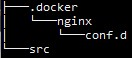
\includegraphics[scale=0.7]{./ressource/arboresence_docker}
\end{center}
\begin{enumerate}[resume]
\item Dans votre fichier d'orchestration copier les lignes ci-dessous : 
\end{enumerate}

\shadowbox{\begin{lstlisting}[language=sh]
#version de docker compose
version: '3.8'
# Services que le veut lancer
services:

  # Service nomme nginx
  nginx:
    #L'image que je veux recuperer
    image: nginx:1.18
    #nom du container
    container_name: nginxPVseul
    #redirection de port
    ports:
      - 80:80
    #repertoires partages
    volumes:
      - ./src:/var/www/html
      - ./.docker/nginx/conf.d/default.d:/etc/nginx/conf.d/default.conf
    #configuration du repertoire de travail  
    working_dir: /var/www/html

\end{lstlisting}}

\paragraph{Les commentaires } (commençant par un '\#') permette de comprendre le rôle des différentes lignes. 

\begin{enumerate}[resume]
\item Dans le fichier de configuration nginx nommé \verb?default.d? placé dans le répertoire créé précédemment \verb?.docker/nginx/conf.d/?, coller les lignes suivantes : 
\end{enumerate}
\shadowbox{\begin{lstlisting}[language=sh]
server {
    listen 80 default_server;
    listen [::]:80 default_server;
    root   /var/www/html;
    index  index.html;


}
\end{lstlisting}}

\begin{enumerate}[resume]
\item Pour lancer le ou les container  à partir d'un fichier   \verb?docker-compose.yml?, il suffit de taper la commande dans le répertoire  : 
\end{enumerate}
\shadowbox{\begin{lstlisting}[language=sh]
docker compose up -d
\end{lstlisting}}


\begin{enumerate}[resume]
\item Pour vérifier que votre container est bien lancé, vous pouvez taper la commande :  
\end{enumerate}
\shadowbox{\begin{lstlisting}[language=sh]
docker compose ps
\end{lstlisting}}

Vous devez alors voir apparaître votre container.

\begin{center}
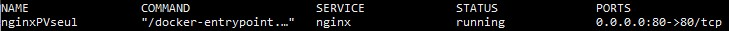
\includegraphics[scale=0.7]{./ressource/resultat_ps.jpg}
\end{center}


\begin{enumerate}[resume]
\item Pour ouvrir un terminal de votre container nginx, vous pouvez tapper la commande  
\end{enumerate}
\shadowbox{\begin{lstlisting}[language=sh]
 docker exec -it nginxPVseul bash
\end{lstlisting}}

\begin{enumerate}[resume]
\item Pour en sortir, il suffit de taper la commande 
\end{enumerate}
\shadowbox{\begin{lstlisting}[language=sh]
exit
\end{lstlisting}}



\subsection{Lemp global}

Pour exécuter le serveur Lemp, il faut compléter (et modifier) le fichier \verb?docker-compose.yml?. L'objectif est de rajouter des services en plus de \verb?nginx?. Par soucis de simplicité, les différents fichiers vous sont donnés (dans le répertoire \verb?ex3-lemp_complet?) : 

\begin{center}
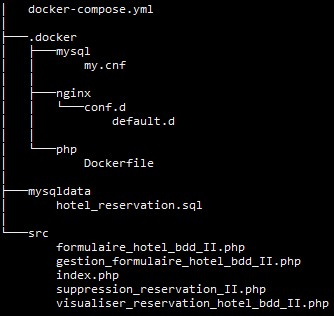
\includegraphics[scale=0.7]{./ressource/arbo_lemp}
\end{center}

\begin{enumerate}
\item Après avoir \textbf{Etudier et commenter} les différents fichiers, activer et tester ce serveur sur docker 
\end{enumerate}

%%%\href{https://tech.osteel.me/posts/docker-for-local-web-development-part-1-a-basic-lemp-stack}{Docker}




\appendix
\newpage
\section{Commendes docker utiles}
\label{lbl_CommandeUtiles}


\paraL{Obtenir les commandes pour docker ou pour docker compose}
\begin{lstlisting}[style=commande]
docker 
\end{lstlisting}

ou 

\begin{lstlisting}[style=commande]
docker compose 
\end{lstlisting}

\paraL{Visualiser les containers en cours d'exécution}

\begin{lstlisting}[style=commande]
docker ps
\end{lstlisting}


\paraL{Visualiser l'ensemble des containers en exécution et arrêtés}

\begin{lstlisting}[style=commande]
docker ps -a
\end{lstlisting}


\paraL{Supprimer un container}

\begin{lstlisting}[style=commande]
docker rm nomDuContainer
\end{lstlisting}

\paraL{Créer une image \verb?nomImage? à partir d'un fichier Dockerfile} (se placer dans le répertoire contenant le fichier\verb?dockerfile?)

\begin{lstlisting}[style=commande]
docker build -t nomimage .
\end{lstlisting}

\paraL{Supprimer une image}

\begin{lstlisting}[style=commande]
docker rmi nomImage
\end{lstlisting}

\paraL{Créer et lancer un conteneur Docker à partir d'une image }

\begin{lstlisting}[style=commande]
docker run [options] <image_name>
\end{lstlisting}



\paraL{Lancer un bash d'un conteneur} 
\begin{lstlisting}[style=commande]
docker exec -it mon_conteneur /bin/bash
\end{lstlisting}



\paraL{Visualiser les logs d'un container} 
\begin{lstlisting}[style=commande]
docker logs nomContainer
\end{lstlisting}

\paraL{Créer et lancer un ensemble de containers à partir de fichier \verb?docker-compose.yml?} (se placer dans le répertoire contenant le fichier\verb?docker-compose.yml?)

\begin{lstlisting}[style=commande]
docker compose up -d
\end{lstlisting}


\paraL{Stopper et supprimer un ensemble de containers} (se placer dans le répertoire contenant le fichier \verb?docker-compose.yml?)
\begin{lstlisting}[style=commande]
docker compose down
\end{lstlisting}

\paraL{Démarrer un ensemble de containers} (se placer dans le répertoire contenant le fichier\verb?docker-compose.yml?)
\begin{lstlisting}[style=commande]
docker compose start
\end{lstlisting}

\paraL{Stopper un ensemble de containers} (se placer dans le répertoire contenant le fichier \verb?docker-compose.yml?)
\begin{lstlisting}[style=commande]
docker compose stop
\end{lstlisting}


\paraL{Partager un volume entre l'hôte et le containers} (dans le fichier \verb?docker-compose.yml?)

\begin{lstlisting}[style=commande]
volumes:
      - ./repHote:repContainer
\end{lstlisting}




\paraL{Rediriger un port dans un container} (dans le fichier \verb?docker-compose.yml?)

\begin{lstlisting}[style=commande]
ports : 
        - 8080:80
\end{lstlisting}
avec 
\begin{itemize}
\itemE 8080 : port hôte
\itemE 80 : port du containers 
\end{itemize}


\end{document}
